\section{Gatling}

Après le projet d'e-banking, j'ai rejoint, avec deux autres stagiaires, Stéphane LANDELLE sur son projet open-source appelé Gatling \cite{gatling} pour le restant de mon stage.

\begin{figure}[H]
 \centering
 
\includegraphics[width=0.3\linewidth]{images/logo_gatling.pdf}
\end{figure}


\subsection{Présentation du projet}

\subsubsection*{Qu'est-ce que Gatling ?}

Gatling \cite{gatling} est un outil permettant de réaliser des tests de charges, par exemple sur des applications web. Ce projet est dans sa grande majorité open-source. Il a été créé par Stéphane LANDELLE, directeur technique d'\ebi{}, en Janvier 2012 et est activement soutenu par le \excilysGroup{}.

Un outil de tests de charge permet de simuler le comportement d'un nombre arbitraire d'utilisateurs pour pouvoir tester le comportement d'une application face à une utilisation simultanée, proche des conditions d'utilisation réelles. Ce type d'outil a pour but de détecter les problèmes de performance d'une application avant sa mise en production.

\subsubsection*{Pourquoi avoir créé Gatling ?}

Avant la création de Gatling il existait déjà de nombreux injecteurs de charge comme :

\begin{itemize}
	\item JMeter
	\item LoadUI
	\item LoadRunner
	\item The Grinder
	\item etc\ldots \\
\end{itemize}

Alors pourquoi créer un nouvel outil ? Car aucun de ceux-ci n'avait satisfait Stéphane LANDELLE lors de ses différentes missions. Il a donc pensé qu'il y avait une place pour un nouvel injecteur qui répondrait à ses attentes.\\

Les principaux inconvénients des solutions existantes sont :

\begin{itemize}
	\item Le coût de la licence pour les solutions payantes : 10000\$ dans le cas de LoadUI.
	\item Le manque d'activité et de maintenance du projet par exemple pour The Grinder. 
	\item Les problèmes de performance de certains outils qui demandent donc une ou plusieurs machines très puissantes pour être efficaces. 
	\item L'écriture des scénarios de tests en XML, ce qui les rend peu lisibles et maintenables, ce qui est le cas de JMeter.\\
\end{itemize}

Gatling a donc été mis au point afin d'offrir une alternative, venant corriger ces problèmes.

\subsubsection*{Qu'est-ce qui différencie Gatling de ses concurrents ?}

Le modèle des \textit{acteurs} sur lequel repose Gatling ainsi que son utilisation des communications asynchrones font de Gatling un outil peu gourmand en ressources.
JMeter, son principal concurrent dans l'écosystème Java, exigera une ou des machines très puissantes pour injecter une charge que Gatling peut effectuer sur une machine aux performances modérées.\\

Une autre différence importante entre Gatling et certains de ses concurrents est le format des scénarios de tests (ou \textit{simulations}).\\
Alors que de nombreux outils utilisent un fichier au format XML afin de décrire leur simulations, ce qui les rend plus difficilement lisibles et manipulables sans passer par l'interface utilisateur de l'outil et également plus difficilement maintenables, les simulations de Gatling sont écrites à l'aide d'un DSL (Domain-Specific programming Language) basé sur Scala, simples à modifier, à mettre à jour et à intégrer au reste du projet (dans le cadre d'un système de contrôle de version par exemple).

\begin{figure}
 \centering
 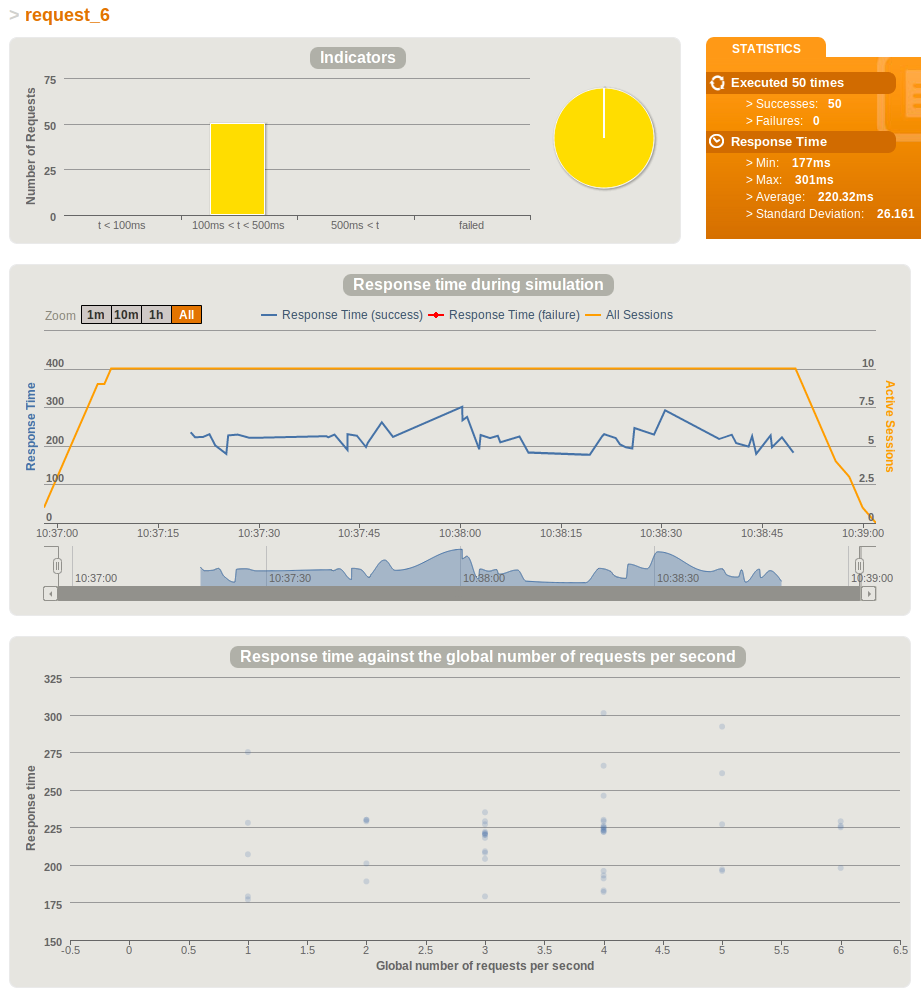
\includegraphics[width=\linewidth]{images/req_details_basic_usage.pdf}
 \caption{Exemple de rapport pour une requête}
\end{figure}

\subsection{Technologies utilisées}

Le projet est lui-même écrit en Scala, un langage de programmation multi-paradigme. Il utilise Akka une librairie Scala/Java permettant de créer facilement des applications concurrentes. Gatling repose pour les I/O sur la librairie Async IO basé sur Netty.

\subsubsection{Scala}

Gatling est écrit en Scala \cite{scala}, un langage qui mélange les paradigmes de programmation orienté objet et de programmation fonctionnelle. Ce langage a été créé en 2003 par Martin ORDERSKY, qui a aussi travaillé sur \verb+javac+, le compilateur Java. Ce langage qui a presque 10 ans connait ces dernières années une augmentation rapide de sa popularité grâce à son utilisation chez Twitter et à la création de frameworks comme Akka ou Play \cite{play} qui permettent de créer des applications web uniquement en Scala.\\

Comme en Java, le code Scala est compilé en bytecode et est exécuté sur une JVM. Scala et Java sont interopérables puisqu'il est possible d'utiliser des API Java en Scala et inversement. D'ailleurs, de nombreuses API du SDK Java n'ont pas d'équivalent en Scala, il suffit d'accéder directement à l'API Java.\\

Scala est un langage fortement typé au même titre que Java, cependant le type des variables peut être inféré à la compilation. De plus il tire beaucoup plus partie de la généricité, c'est à dire le fait de paramétrer une classe ou une fonction par un type. L'objectif étant d'avoir un maximum d'erreur de type découvert par le compilateur et non à l'exécution.\\

Un des avantages de Scala est l'écriture d'un code beaucoup plus concis qu'en Java, au prix d'une compilation plus lente. Le code Scala est plus concis car il permet d'éviter d'écrire toute la partie du code qui n'est pas réellement utile et qui devient donc facultative.\\

Ce langage permet d'écrire un code vraiment réduit à son essence, ce qui permet de le rendre plus maintenable. Sa compréhension peut être cependant plus complexe. De plus, la façon de développer et penser son code est différente de celle de Java puisqu'on est aussi dans un paradigme de programmation fonctionnelle.\\

Il a donc nécessité un temps d'adaptation et d'apprentissage \cite{proginscala} avant de pouvoir comprendre le fonctionnement interne de Gatling et de pouvoir développer de nouvelles fonctionnalités.

\subsubsection{Akka}

Akka \cite{akka} est un framework écrit en Scala, disposant aussi d'une API Java, pour faciliter la réalisation d'applications fortement concurrentes en s'appuyant sur le système des Acteurs. Le framework Akka permet de s'abstraire de la notion de threads et d'exploiter au maximum les processeurs multi-cœurs. Dans le cas de Gatling, l'objectif est de pouvoir gérer un grand nombre d'utilisateurs en parallèle.\\

Akka utilise, pour s'abstraire des threads et régler les problèmes de synchronisation liés à la concurrence, le système des acteurs. Les acteurs sont des objets encapsulant un état et un comportement. Ils communiquent entre eux exclusivement à l'aide de messages placés dans une boite aux lettres propre à chaque acteur. L'exécution d'un acteur est démarré par la réception d'un message. Ceci permet de réaliser la plupart des traitements de manière asynchrone et de minimiser ainsi le blocage des threads. En effet un acteur n'est pas lié à un thread, il est exécuté sur un thread quelconque lorsque cela est nécessaire. En interne, Akka utilise un pool de threads pour exécuter les acteurs. Ceci permet d'avoir potentiellement un très grand nombre d'acteurs qui s'exécutent (plus de 1000) sur un pool de threads restreints (30 threads).

\subsubsection{Netty \& Async HTTP Handler}

Async HTTP Handler est un client HTTP reposant sur le moteur Netty qui permet de gérer l'envoi de requêtes (et le traitement des réponses) HTTP de manière asynchrone, complétant ainsi le caractère asynchrone d'Akka, ce qui permet à Gatling de disposer d'un moteur intégralement asynchrone. 

\subsection{Architecture de Gatling}

\begin{center}
	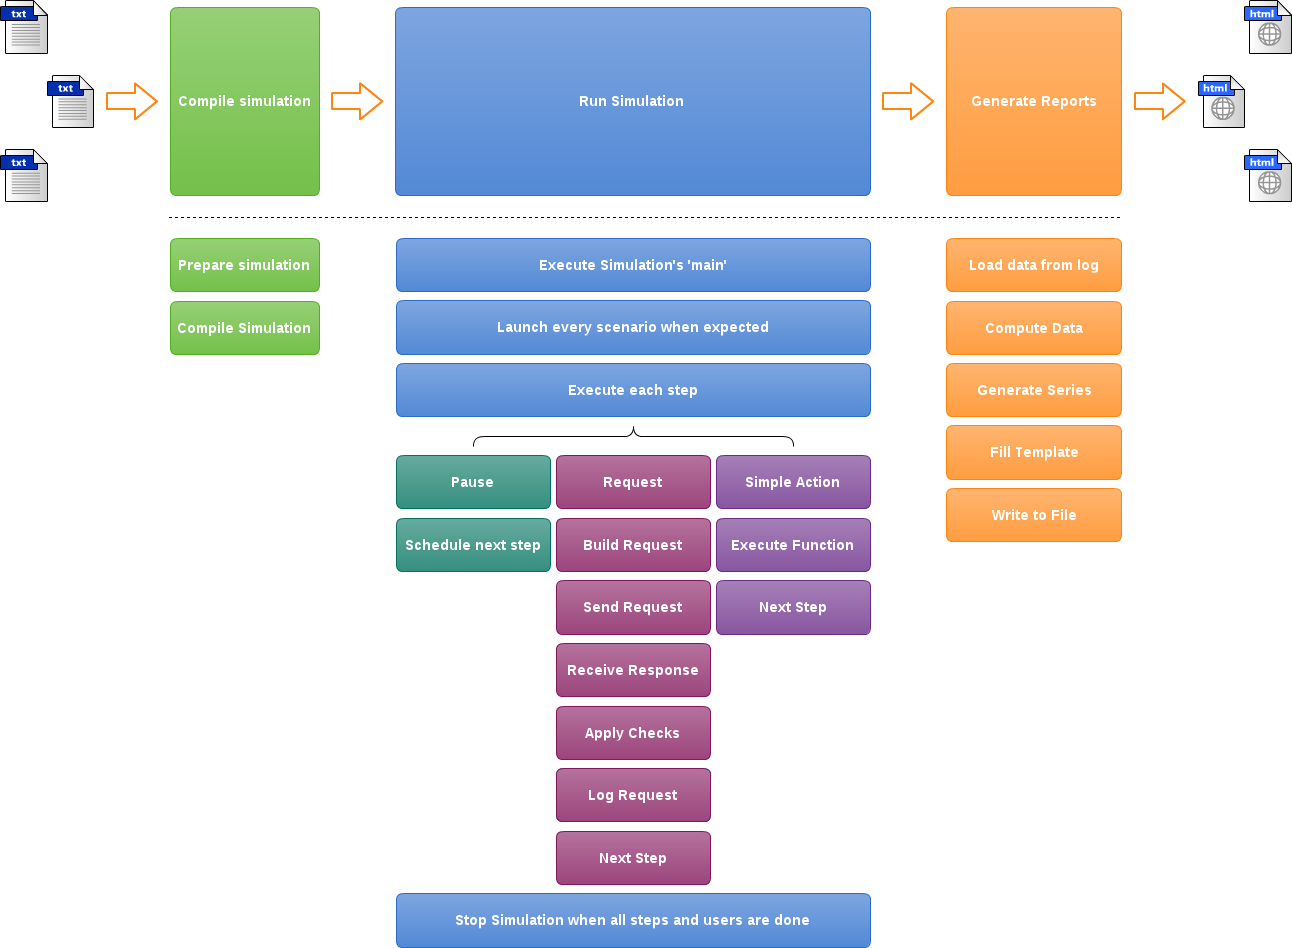
\includegraphics[scale=0.3]{images/gatling-process.pdf}
\end{center}

\subsection{Récupération des métriques serveurs}

Actuellement, les mesures prises par Gatling ne concernent que ce qu'un utilisateur de l'application observerait : le temps que met une page web à répondre ou tout simplement si celle-ci répond ou non.\\

La première fonctionnalité que Stéphane LANDELLE souhaitait que nous étudions était le monitoring de l'application testée, côté serveur.\\

Ce choix était motivé par deux raisons :

\begin{itemize}
	\item Bien qu'étant open source, Gatling reste en concurrence avec d'autres solutions, et plusieurs d'entre elles proposent du monitoring côté serveur ou comptent en intégrer dans un futur proche. Intégrer du monitoring c\^oté serveur  dans Gatling permettrait donc à celui-ci de ne pas prendre de retard sur la concurrence.
	\item Monitorer l'application testée permettrait d'obtenir de précieuses informations sur le comportement de l'application durant le test que ça soit en terme d'utilisation CPU, de mémoire, d'activité des bases de données\ldots En recoupant ces informations avec celles déjà existantes, cela permettrait d'obtenir des rapports encore plus pertinents.\\
\end{itemize}

Pour pouvoir mettre en place cette fonctionnalité, nous avons donc effectué un état de l'art des technologies à utiliser, puis nous les avons testées pour vérifier leur impact sur les performances du serveur instrumenté (cf. annexe~\ref{ann:benchmark}).\\

\subsubsection{Java Management eXtensions}

La première technologie que nous avons trouvée est Java Management eXtensions (JMX) \cite{jmx}. JMX est une API Java qui permet de gérer à distance des applications s'exécutant sur une JVM. Elle permet de récupérer des informations exposées par JMX telles que l'utilisation du CPU par la JVM, mais elle permet aussi d'appeler des méthodes distantes pour, par exemple, redémarrer des composants.\\

En interne, JMX repose sur RMI (Remote Method Invocation), une API Java qui permet d'appeler des méthodes sur des objets distants. L'utilisation de JMX est extrêmement simple, puisqu'il suffit de créer une interface dont le nom se termine par \verb+MBean+ ainsi qu'une classe implémentant cette interface. Elle sera alors automatiquement exposée par JMX et accessible de l'extérieur.\\

Pour pouvoir facilement accéder aux objets exposés (appelés MBean), nous avons utilisé JVisualVM, un programme fournit avec le JDK (Java Development Kit) d'Oracle. Ce programme permet de monitorer des JVM locales ou distantes en accédant notamment aux MBean.

\begin{figure}[H]
 \centering
 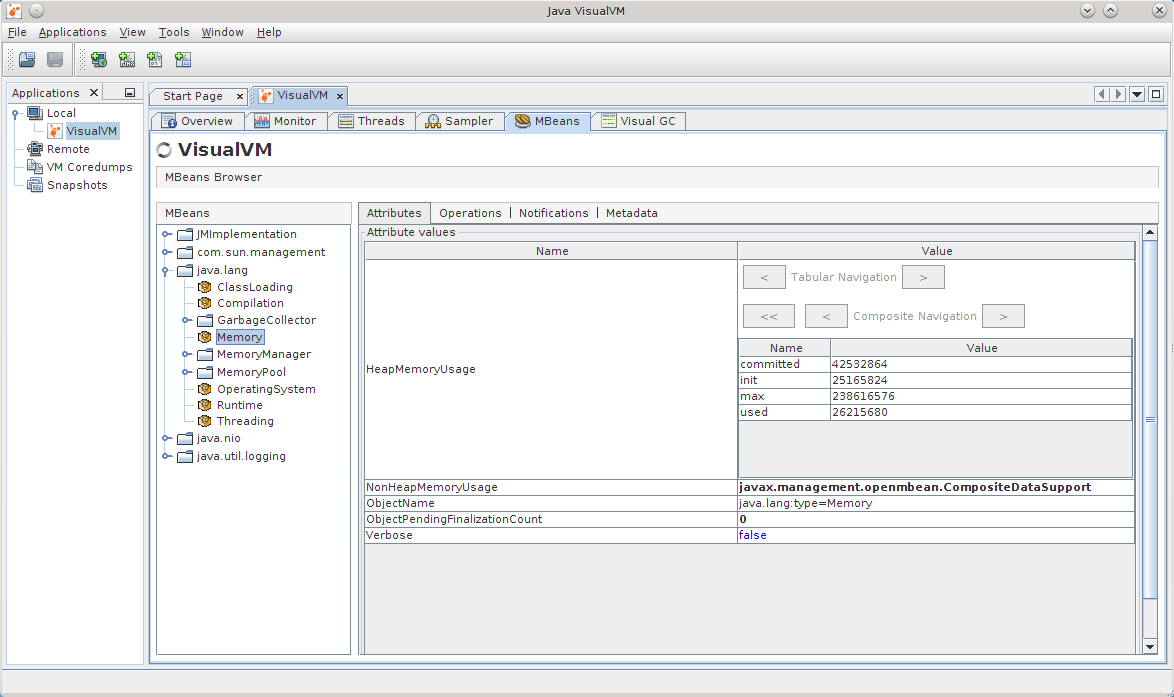
\includegraphics[width=\linewidth]{images/jvisualvm.pdf}
 \caption{Utilisation de JVisualVM pour accéder aux MBean}
\end{figure}


L'utilisation de JMX est donc très simple, de plus, plusieurs métriques sont déjà exposées par la JVM, telle que l'utilisation du \textit{CPU}, l'utilisation de la \textit{Heap} (mémoire interne de la JVM), la durée totale de collecte par le Garbage Collector (GC), \dots{}\\

Cependant, un des inconvénients de l'utilisation de JMX est l'utilisation sous-jacente de RMI qui déclenche régulièrement le GC. L'exécution de celui-ci étant coûteuse en performance, son utilisation peut avoir un impact sur le serveur testé et ainsi fausser les résultats du test de charge.

\subsubsection{Agent Java}

La deuxième technologie est l'utilisation d'un agent java. Un agent java est un code Java qui est exécuté au démarrage de la JVM avant la méthode \verb+main+. Un agent permet notamment de manipuler le bytecode d'une classe au chargement de celle-ci. On peut aussi utiliser un agent pour exécuter du code en parallèle de l'application et donc par exemple, écrire dans un fichier les métriques que l'on veut récupérer.\\

Un des inconvénients des agents est qu'il faut modifier la ligne de commande qui démarre le serveur pour pouvoir ajouter notre agent. Son utilisation est donc assez complexe puisqu'il nécessite une intervention de la personne qui souhaite utiliser Gatling.\\

Cependant, Sun a créé une API permettant d'attacher un agent à une JVM déjà en cours d'exécution. Il est donc possible d'attacher notre code à une JVM de façon assez simple. Cette API possède une limitation puisqu'on ne peut attacher un agent uniquement à une JVM locale et non distante. Son utilisation nécessite donc toujours une intervention de l'utilisateur de Gatling, mais l'intervention est plus simple puisqu'il ne s'agit que d'exécuter un programme qui va découvrir les JVM et attacher l'agent.\\

Un agent permet donc d'exécuter notre code et donc de créer des sondes qui vont permettre d'enregistrer ou d'envoyer à une application tierce, les métriques que l'on souhaite récupérer. Ces sondes peuvent bien évidemment tirer partie de JMX pour exposer les métriques.

\subsubsection{Sigar}

Nous nous sommes ensuite renseignés sur des API permettant de récupérer des informations de la machine elle-même. Cette partie est plus complexe puisqu'elle est dépendante du système d'exploitation. Nous avons alors trouvé Sigar développé par Hyperic \cite{sigar}.\\

Sigar répond tout à fait à la problématique puisqu'il propose une API indépendante du système d'exploitation mais fonctionnant à la fois sur Windows, Mac OS X, Linux, \dots{} Il utilise JNI (Java Native Interface) pour faire appel à des librairies écrites en C dépendantes, elles, du système d'exploitation.\\

Son utilisation assez simple a un inconvénient : la librairie correspondante au système d'exploitation doit être accessible par le code qui utilise Sigar. Il faut donc que l'utilisateur de Gatling installe Sigar sur le système contenant le serveur.\\

Cependant, si on considère l'utilisation de Sigar avec un agent, il suffit de mettre dans l'archive contenant l'agent, toutes les librairies pouvant être utilisées. Son utilisation est donc envisageable.

\subsubsection{Metrics}

Le dernier point sur lequel nous avons fait des recherches est sur la façon d'enregistrer les métriques du serveur. À la fin de l'exécution du test de charge, les métriques doivent être mises à disposition de Gatling, c'est la seule contrainte.\\

Nous avons donc envisager plusieurs solutions :

\begin{itemize}
 \item Écrire dans un fichier puis l'envoyer à Gatling à la fin du test,
 \item Écrire dans une base de donnée SQL ou NoSQL distante,
 \item Envoyer les données au fur et à mesure à Gatling.\\
\end{itemize}

Les deux dernières solutions consomment de la bande passante ce qui est un sérieux inconvénient puisque le trafic vers le serveur est sûrement surchargé à cause du test. La première solution, quand à elle, risque d'impacter les performances côté serveur à cause des accès disques.\\

Nous nous sommes alors rendu compte que ces solutions pouvait dépendre du cas d'utilisation et qu'il était plus intelligent de laisser le choix à l'utilisateur de Gatling. Il nous fallait donc un système qui permette de s'abstraire de la méthode d'enregistrement des résultats. Pour cela, nous avons décidé d'utiliser Metrics \cite{metrics}, développé par Yammer, une plateforme de réseaux sociaux privés pour les entreprises.\\

Metrics permet de consolider des données sous forme de statistiques, c'est à dire sous la forme d'une simple valeur, d'un compteur, d'un histogramme, \dots{} Metrics permet aussi d'envoyer régulièrement ces statistiques vers différents systèmes : un fichier, des applications de monitoring tierces (Graphite, Ganglia), via JMX \dots{}\\

Avec Metrics, il est aussi possible de créer notre propre système d'écriture des données pour envoyer les statistiques vers une base de données par exemple.

\subsubsection{Notre solution}

La solution que nous avons prototypé mais pas développé est la suivante : nous utilisons un agent que nous attachons au serveur via l'API Attach. Cet agent accède aux informations de la JVM via JMX en local et aux informations de la machine via Sigar. Les données sont consolidées par Metrics et enregistrées via un système configurable : écriture dans un fichier ou dans une base de données.\\

Nous n'avons pas développé cette solution pour plusieurs raisons :
\begin{itemize}
 \item Elle impacte les performances du serveur en test et fausse donc les résultats,
 \item Notre problématique se rapproche beaucoup du monitoring d'un serveur pour lequel il existe déjà des solutions plus performantes et complètes.\\
\end{itemize}

Cette fonctionnalité n'avait donc pas vraiment sa place dans Gatling.

\subsection{Exposition des métriques Gatling}

Si la précédente fonctionnalité n'a pas été développée, elle a donné l'idée d'exposer les statistiques de Gatling pour être accessibles à un système tiers. En effet, pour le monitoring de serveur, des applications telles que Graphite et Ganglia sont très utilisées. L'objectif était donc de consolider un certain nombre de métriques en temps réel et de les envoyer vers ces systèmes.\\

Je n'ai que très peu travaillé sur cette fonctionnalité, je ne m'étendrai donc pas dessus.

\subsection{Génération des rapports}

Je suis ensuite passé sur une troisième fonctionnalité. Cette fonctionnalité est une amélioration d'une partie de Gatling et est due à une remarque d'un utilisateur. Cet utilisateur a testé son application pendant 48 heures générant un journal de 8 Go à traiter pour créer le rapport. Cependant cette génération de rapport nécessitait le chargement du fichier en mémoire ce qui n'était dans le cas présent pas possible.\\

Pour mieux comprendre, voici le fonctionnement de Gatling :
\begin{enumerate}
 \item Compilation du scénario de test,
 \item Exécution des requêtes du scénario. Chaque exécution génère une ligne dans le journal contenant des informations brutes telles que le succès ou l'échec de la requête, le nom de la requête, l'heure de début et de fin de la requête, l'heure de début et de fin de la réponse,
 \item Lorsque le scénario est fini, le journal est traité pour générer le rapport final.\\
\end{enumerate}

Il y a plusieurs avantage à cette méthode :
\begin{itemize}
 \item Il n'y a pas de perte de performances due au calcul de statistiques pendant le test,
 \item Si Gatling plante, peu importe la raison, les données ne sont pas perdues car écrites au fur et à mesure. Il est possible alors de relancer Gatling uniquement pour générer le rapport.\\
\end{itemize}

Comme expliqué précédemment la méthode utilisée auparavant chargeait tout le fichier en mémoire pour pouvoir le traiter. En effet, c'est la méthode la plus simple pour pouvoir déterminer des statistiques telles que les quantiles (médiane, 95\ieme{} percentile, 99\ieme{} percentile).\\

Nous nous sommes donc renseignés sur les systèmes permettant de traiter des quantités importantes de données sans avoir besoin de charger en mémoire toutes les données et ainsi réduire de façon significative la mémoire utilisée.

\subsubsection{MapReduce}

Popularisé par Google, MapReduce est un modèle de programmation permettant de traiter de façon parallèle et distribuée une quantité importante de données (du téraoctet au pétaoctet). MapReduce modélise la chaîne de traitement des données par une succession de tâches \verb+map+ et \verb+reduce+.\\

Une tâche \verb+map+ correspond à un traitement donnée par donnée. Voici la signature en pseudo-code de la fonction \verb+map+ :

\begin{center}
 \verb+map(key: K1, value: V1): (K2, V2)+
\end{center}

Cette fonction permet donc d'appliquer un traitement à chaque paire clé/valeur pour renvoyer une paire clé/valeur. Les types ne sont pas forcément identiques. La tâche \verb+reduce+ permet à partir d'un ensemble de données de calculer un résultat unique :

\begin{center}
 \verb+reduce(key: K, values: List<V1>): V2+
\end{center}

Une telle fonction permet de regrouper toutes les valeurs dont la clé est identique et de calculer un résultat unique.\\

L'idée de MapReduce est de ne simplement écrire que les tâches \verb+map+, \verb+reduce+ et leur enchaînement. Le système s'occupe de diviser les données en entrée en petites unités, exécuter les différentes tâches en parallèles et de manière distribuée sur ces unités, regrouper les données pour les tâches \verb+reduce+, \dots{}\\

Cette méthode de calcul n'étant qu'une méthode, nous avons cherché comment la mettre en place pour voir si elle est utilisable dans notre cas.

\subsubsection{Apache Hadoop}

Une des implémentations open source de MapReduce est le projet Apache Hadoop \cite{hadoop}. Il propose une API simple pour créer les tâches puisqu'il suffit simplement d'implémenter les interfaces Mapper et Reducer. Hadoop repose sur un système de fichier distribué appelé HDFS pour pouvoir s'exécuter en parallèle dans un cluster de machines.\\

De toute évidence, nous ne cherchions pas à effectuer des calculs distribués, nous nous sommes donc pencher sur une utilisation simpliste de Hadoop en local. Mais nous avons trouvé que l'écriture de tâches \verb+map+ et \verb+reduce+ était assez complexe et surtout très verbeuse car de bas niveau.\\

Nous avons donc cherché des librairies d'abstraction à Hadoop pour nous simplifier le travail.

\subsubsection{Cascading et Scalding}

Il existe plusieurs librairies d'abstraction, certaines plus abouties que d'autres. Celle que nous avons retenue s'appelle Cascading, c'est la solution la plus répandue, elle est entre autre utilisée en production par Twitter. Ces derniers ont développé une sur-couche à Cascading en Scala, Scalding, que nous avons aussi utilisée car elle rend l'écriture des tâches plus aisée. Ces solutions offrent des traitements comme le GroupBy au sens SQL, \dots{}\\

Un autre avantage de Cascading est son mode local qui ne s'appuie pas sur Hadoop mais sur une implémentation intelligente en mémoire dont l'objectif est de tester les traitements en Cascading. Bien qu'à des fins de tests nous nous sommes intéressés à l'utilisation de ce mode pour notre problématique. Nous avons donc testé ce mode local pour en comprendre le fonctionnement et les limites.\\

Après ces tests, nous avons pu comprendre les limites de ce mode local. La limite principale n'est pas tellement la taille du fichier en entrée mais le nombre de données intermédiaires. En effet, le mode local est suffisamment intelligent pour exécuter un maximum de calcul au fur et à mesure de la lecture du fichier. Le seul traitement bloquant étant un \verb+reduce+ qui a besoin de toutes les données pour avoir le résultat. Cependant, un \verb+reduce+ n'a pas besoin de toutes les données en mémoire pour s'exécuter, les calculs peuvent passer par des résultats partiels.\\

Pour mieux comprendre son fonctionnement, voici un exemple de traitement :
\begin{figure}[H]
	\centering
	\includegraphics[width=0.7\textwidth]{images/cascading.pdf}
\end{figure}

Ce traitement est simple : pour chaque ligne, on calcul la différence entre \verb+c+ et \verb+b+, puis on regroupe par \verb+a+. Pour chaque groupe, on calcul le moyenne de \verb+d+. Avec le mode local de Cascading, ce calcul s'effectue en une étape : à chaque ligne, on applique la tâche \verb+map+, puis on calcul le résultat partiel pour la tâche \verb+reduce+. Voici le schéma pour mieux comprendre :

\begin{figure}[H]
	\centering
	\includegraphics[width=0.7\textwidth]{images/cascading_real.pdf}
\end{figure}

Ainsi tout le fichier n'est pas en mémoire. Bien sûr, pour que dans notre exemple le résultat soit juste pour plus de données, il faut avoir le nombre de données nécessaires pour calculer un résultat partiel pour pouvoir calculer le suivant. Cette donnée intermédiaire n'est pas représentée mais est bien présente.\\

Cascading va donc fusionner les tâches \verb+map+ entre chaque tâche \verb+reduce+ et calculer cette dernière au fur et à mesure. Les résultats en mémoire ne seront donc que les résultats des \verb+reduce+ intermédiaires. Il y a bien sûr des cas où il faut toutes les données en mémoires : la fonction utilisée pour le \verb+reduce+ n'est pas associative, c'est à dire que l'ordre d'application pour réduire une liste de données à un résultat dépend de l'ordre des données en entrée.\\

De plus, dans la mesure ou les résultats des \verb+reduce+ intermédiaires est en mémoire, il faut qu'ils puissent tenir en mémoire. Le comportement du mode local de Cascading dépend donc des calculs. Dans notre cas, la librairie utilisée pour afficher les résultats n'affiche pas plus de 5000 points par courbe. La première étape du calcul est donc de regrouper les données par nom de la requête, status de la requête (succès ou échec) et par intervalle de temps. La taille de ces intervalles étant calculée de façon qu'il n'y en ait pas plus de 5000. La nature de nos calculs fait que quelque soit la taille du fichier en entrée les résultats intermédiaires ont une empreinte mémoire très faible (moins de 200 Mo pour un test de 48h représentant un journal de 8Go).\\

\subsubsection{Développement de l'amélioration}

Pour mettre en place l'amélioration, nous avons commencé par développer une application \textit{standalone} qui permet de générer le rapport à partir du journal. Cette application effectue un traitement en 3 phases :

\begin{enumerate}
 \item Lecture complète du fichier pour déterminer des valeurs générales nécessaires au traitement, notamment l'heure de début et l'heure de fin du test. Ces deux valeurs vont permettre de déterminer la taille des intervalles de temps pour ne garder que 5000 valeurs au plus pour les graphiques.
 \item Traitement avec Scalding utilisant Cascading en mode local, ce qui permet de calculer la quasi-totalité des données statistiques.
 \item Calcul des dernières statistiques notamment les quantiles et le nombre de sessions actives par classe au cours du test. Ces calculs nécessitent de parcourir une liste de valeur dans un ordre précis avec une connaissance de la précédente valeur, ce qui n'est pas possible en MapReduce. Ainsi, on calcule la distribution des valeurs à l'étape 2 puis nous déterminons les quantiles à partir de cette distribution. De même, pour les sessions actives, l'étape 2 détermine le nombre de sessions actives en plus ou en moins par intervalle de temps. Cette 3\ieme{} étape fait la synthèse des données pour avoir le nombre de sessions actives par classe.\\
\end{enumerate}

Une fois l'ensemble des statistiques calculées avec notre méthode, nous l'avons testée avec un journal de 8 Go. Le calcul du résultat a demandé 14 minutes avec une empreinte mémoire de moins de 200 Mo. L'empreinte mémoire a été déterminée avec JVisualVM qui permet d'afficher l'utilisation de la mémoire d'une JVM en cours d'exécution. Les 14 minutes correspondent au temps nécessaire pour lire le fichier 2 fois. Les calculs étant plus rapides que la lecture sur disque, il est donc normal que la partie bloquante soit la lecture.\\

Nous avons ensuite intégré notre travail dans Gatling, en remplaçant l'implémentation actuelle de la génération du rapport par la nôtre. Notre travail a été intégré à la branche \textit{master} de Gatling et est présente dans la release 1.3.0 sortie le 20 septembre.

\subsubsection{Conclusion}

L'utilisation de Cascading en mode local, nous aura permis de comprendre la nécessité de tester les frameworks que l'on pourrait utiliser. En effet, notre utilisation de Cascading en production n'est pas recommandée car nous utilisons une partie qui normalement sert de test. C'est cependant à mettre en perspective par rapport à l'utilisation en production : Cascading sert à traiter des téraoctets de données. La volumétrie est donc importante ici puisque dans notre cas nous ne traitons que des journaux de quelques gigaoctets au maximum.\\

Scalding s'est avéré être très utile car l'écriture du traitement est beaucoup moins verbeuse et plus intuitive qu'en Cascading, cependant, cette librarie créée par Twitter est très mal conçue car elle dépend fortement de Hadoop, même si on utilise le mode local de Cascading. On est donc obligé d'avoir une dépendance à Hadoop bien que nous ne l'utilisons pas.

\subsection{Plugin Jenkins}

Le dernier chantier auquel j'ai participé est la conception et la réalisation d'un plugin Jenkins permettant d'intégrer le suivi d'une simulation Gatling.\\

Jenkins \cite{jenkins}, anciennement Hudson, est le serveur d'intégration le plus utilisé dans le monde Java. Un tel outil permet de récupérer les source du projet sur un dépôt distant, de construire le projet, par exemple à l'aide de Maven, et enfin de réaliser un certain nombre d'actions en fonction de la réussite ou non de la construction du projet. Tout ce processus peut être planifié par exemple à chaque \textit{push} sur le système de gestion de versions ou à heure fixe.

Une des grande force de Jenkins est la possibilité de réaliser des plugins pour celui-ci, ce qui le rend modulaire et personnalisable.\\ 

La réalisation de ce plugin a été motivée par plusieurs raisons :

\begin{itemize}
	\item Le principal concurrent de Gatling, JMeter, offre une telle intégration à Jenkins au travers du Performance Plugin \cite{perfplugin}, qui compte plus de 2500 utilisateurs.
	\item Gatling offre déjà un plugin Maven qui permet de lancer une simulation lors du build. Ainsi offrir le suivi de celle-ci dans Jenkins est une évolution logique.
	\item Enfin cette intégration est demandée depuis un certain temps par la communauté d'utilisateurs de Gatling.
\end{itemize}

\subsubsection{Conception}

La première piste que nous avons explorée a été non pas de réaliser un nouveau plugin mais d'intégrer Gatling au Performance Plugin déjà existant. Pour pouvoir réalisé ceci, il fallait écrire le journal Gatling au format de celui de JMeter. Cette étape a été relativement facile à réaliser. Nous avons donc eu rapidement une intégration de Gatling dans Jenkins. Cependant en testant cette solution nous nous sommes rendus compte que le Performance Plugin avait de graves problèmes de performance. Celui-ci était fonctionnel seulement si le journal généré était de très petite taille, de l'ordre de quelques méga-octets. Cette solution n'était donc pas viable.\\

La seconde piste que nous avons étudié a été la réalisation d'un plugin Jenkins entièrement dédié à Gatling.
En s'inspirant du Performance Plugin et en prenant en compte les désirs des utilisateurs de Gatling nous avons identifié les fonctionnalités suivantes comme primordiales :

\begin{itemize}
	\item Pouvoir définir des conditions d'échec ou d'instabilité de la build en fonction  des résultats de la simulation Gatling.
	\item Pouvoir visualiser l'évolution des performances de l'application au cours du temps.
	\item Pouvoir accéder aux rapports Gatling directement dans l'interface de Jenkins.
\end{itemize}

\subsubsection{Réalisation}

Nous avons donc réalisé ces trois fonctionnalités. La réalisation du plugin n'a pas été aisée en raison du manque criant de documentation. Jenkins ainsi que ses plugins s'appuie sur des technologies développées par son créateur  Kohsuke Kawaguchi. Ces technologies sont peu utilisées, à part dans Jenkins, et surtout peu documentées alors même qu'elles s'appuient sur le principe de \textit{convention over configuration}.

La réalisation du plugin se fait en implémentant les interfaces adéquates. Chaque interface permettant d'étendre un comportement. Le framework web utilisé par Jenkins est Stapler \cite{stapler}, l'outil pour réalisé les vues est Jelly \cite{jelly}. L'écriture d'un plugin nécessite l'utilisation de ces outils et leur compréhension.

Pour réaliser les différents graphiques nous avons décidé de ne pas nous appuyer sur la solution intégrée à Jenkins, qui se base sur JFreeChart, mais de plutôt utiliser jQPlot \cite{jqplot}, un plugin jQuery, qui permet de faire des graphiques plus dynamiques et plus beau.

\subsubsection{Résultat}

Le plugin Jenkins que nous avons développé est actuellement fonctionnel (cf. annexe~\ref{ann:jenkins}). Il devrait être prochainement testé par des utilisateurs. Ce qui nous permettra de réaliser quelques ajustements. Ce projet n'est pas directement intégré au projet Gatling, mais est à part \cite{gatlingplugin}, ce qui lui permettra d'évoluer en parallèle de Gatling. 